% !TEX encoding = IsoLatin9
\section{La machine de Turing}\label{section:2}
\begin{frame}
  \begin{columns}
    \column{4.8cm}
    \tableofcontents[currentsection,hideothersubsections]
    \column{7cm}
    \centering{
      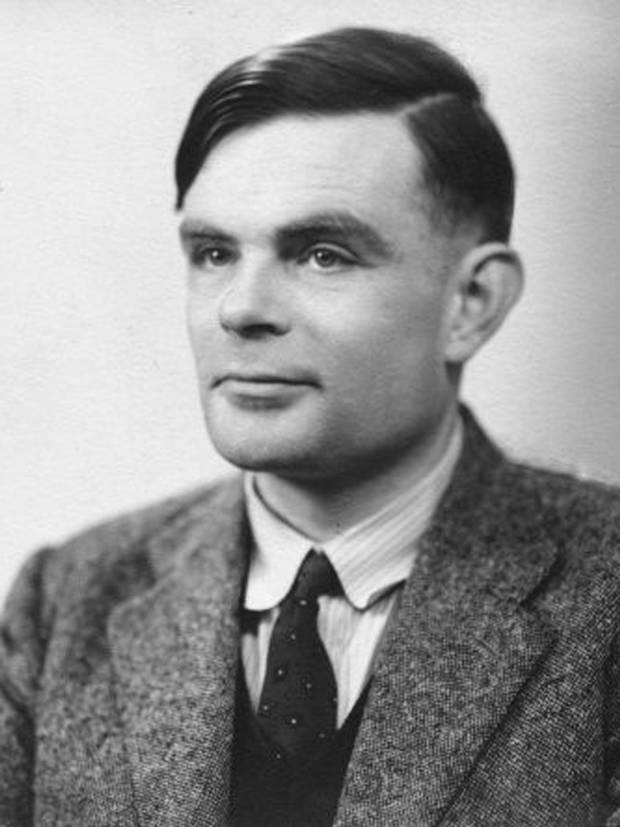
\includegraphics[width=4cm]{fig/turing.jpg}
      
      \textit{``A computer would deserve to be called intelligent
if it could deceive a human into believing that it was human.''}\\
      \small{
        \hfill Alan Turing (1912-1954) 
              }
    }
  \end{columns}
  
\end{frame}

\begin{frame}
\frametitle{Un peu d'histoire...}
\begin{description}
%[font=\color{red}]
\item[1900 : ]Probl�mes d'Hilbert (2�me probl�me : Est-ce que l'arithm�tique est coh�rente ?)\\
\item[1931 : ]G�del d�montre que l'arithm�tique est incompl�te. Cela est li� au probl�me de la d�cision.\\
\item[1936 : ]Introduction de la machine de Turing par Alan Turing � l'�ge de 24 ans pour montrer
que certais probl�mes ne peuvent pas �tre r�solus par un algorithme (c'est � dire par la machine de Turing).\\
\item[1942 : ]Participation au d�codage d'Enigma.\\
\item[1946 : ]Cr�ation de l'ENIAC (Electronic Numerical Integrator and Computer).\\
\item[1954 : ]Mort de Turing.
\includegraphics[scale=0.03]{./fig/apple.jpg}\\
\end{description}
\end{frame}

\begin{frame}
\frametitle{D�finition de la machine de Turing}
\begin{columns}

\column{.4\textwidth}
\begin{enumerate}
\item<1-|alert@1> Un ruban infini contenant des symboles. \tikz[remember picture,baseline=-.5ex] \coordinate(it1);
\item<2-|alert@2> Un t�te de lecture/�criture. \tikz[remember picture,baseline=-.5ex] \coordinate(it2);
\item<3-|alert@3> Un registre d'�tat. \tikz[remember picture,baseline=-.5ex] \coordinate(it3);
\item<4-|alert@4> Une table d'actions. \tikz[remember picture,baseline=-.5ex] \coordinate(it4);
\item<5-|alert@5> Un �tat et une position de d�part sur le ruban.\\
\end{enumerate}
\column{.55\textwidth}
\begin{figure}
\centering
\begin{tikzpicture}[remember picture]
\tikzstyle{every path}=[very thick]

\edef\sizetape{0.7cm}
\tikzstyle{tmtape}=[draw,minimum size=\sizetape]
\tikzstyle{tmhead}=[arrow box,draw,minimum size=.5cm,arrow box
arrows={east:.25cm, west:0.25cm}]

%% Draw TM tape
\begin{scope}[start chain=1 going right,node distance=-0.15mm]
    \node [on chain=1,tmtape,draw=none,xshift=1mm] {\tiny{$\ldots$}};
    \node [on chain=1,tmtape] {0};
    \node [on chain=1,tmtape] {1};
    \node [on chain=1,tmtape] {1};
    \node [on chain=1,tmtape] {0};
    \node [on chain=1,tmtape] (input){0};
    \node [on chain=1,tmtape] {0};
    \node [on chain=1,tmtape] {0};
    \node [on chain=1,tmtape] {0};
    \node [on chain=1,tmtape,draw=none,xshift=-1mm] (right) {\tiny{$\ldots$}};
\end{scope}
\node [tmhead,yshift=-.3cm] at (input.south) (head) {$e_1$};
\end{tikzpicture}
\end{figure}


\end{columns}
\begin{table}
\footnotesize
\begin{tabular}{|c|c|c|c|c|}
\hline
\textbf{Ancien �tat} & \textbf{Symbole lu} & 
\textbf{Symbole\tikz[remember picture,baseline=-1ex] \coordinate(tab);   �crit} & \textbf{Mouvement} &   \textbf{Nouvel �tat} \\
\hline
& & & &\\
\end{tabular}
\end{table}

\begin{tikzpicture}[remember picture,overlay,scale=0.8]
\draw <1|handout:0> (it1) edge[bend left, ->, very thick,shorten >=2pt,color=red ] (input.north);
\draw <2-> (it1) edge[bend left, ->, very thick,shorten >=2pt ] (input.north);

\draw<2|handout:0> (it2) edge[bend right, ->, very thick,shorten >=2pt,color=red] (head.west) ;
\draw<3-> (it2) edge[bend right, ->, very thick,shorten >=2pt] (head.west) ;

\draw<3|handout:0> (it3) edge[bend right, ->, very thick,shorten >=5pt,color=red] (head.center) ;
\draw<4-> (it3) edge[bend right, ->, very thick,shorten >=5pt] (head.center) ;

\draw<4|handout:0> (it4)   edge[bend left, ->, very thick,shorten >=5pt,color=red](tab);
\draw<5-> (it4)   edge[bend left, ->, very thick,shorten >=5pt](tab);
\end{tikzpicture}

\end{frame}


\begin{frame}
\frametitle{Fonctionnement d'une machine de Turing}
\begin{columns}

\column{.4\textwidth}

\begin{enumerate}
\footnotesize
\item<1-|alert@1>La t�te de lecture lit un symbole $s$. \tikz[remember picture,baseline=-.5ex] \coordinate(it1);
\item<2-|alert@2>En fonction de $s$ et de son �tat, la t�te �crit un symbole $s'$ \tikz[remember picture,baseline=-.5ex] \coordinate(it2);
\item<3-|alert@3>En fonction de son �tat la t�te se d�place d'un cran.  \tikz[remember picture,baseline=-.5ex] \coordinate(it3);
\item<4-|alert@4>La machine change d'�tat. \tikz[remember picture,baseline=-.5ex] \coordinate(it4);
\end{enumerate}


\column{.55\textwidth}
\begin{figure}
\centering
\begin{tikzpicture}[remember picture]
\tikzstyle{every path}=[very thick]

\edef\sizetape{0.7cm}
\tikzstyle{tmtape}=[draw,minimum size=\sizetape]
\tikzstyle{tmhead}=[arrow box,draw,minimum size=.5cm,arrow box
arrows={east:.25cm, west:0.25cm}]

%% Draw TM tape
\begin{scope}[start chain=1 going right,node distance=-0.15mm]
    \node [on chain=1,tmtape,draw=none,xshift=1mm] {\tiny{$\ldots$}};
    \node [on chain=1,tmtape] {0};
    \node [on chain=1,tmtape] {0};
    \node [on chain=1,tmtape] {0};
    \node [on chain=1,tmtape] {0};
    \node [on chain=1,tmtape] (input){\alt<2-|handout:0>{\textcolor<2>{red}{1}}{\textcolor<1>{red}{0}}};
    \node [on chain=1,tmtape] (step) {0};
    \node [on chain=1,tmtape] {0};
    \node [on chain=1,tmtape] {0};
    \node [on chain=1,tmtape,draw=none,xshift=-1mm] (right) {\tiny{$\ldots$}};
\end{scope}
\visible<1-2> {\node [tmhead,yshift=-.3cm] at (input.south) (head) {$e_1$};}
\visible<3-|handout:0> {\node [tmhead,yshift=-.3cm] at (step.south) (head) {\alt<4->{\textcolor{red}{$e_2$}}{$e_1$}};}

\end{tikzpicture}
\end{figure}


\end{columns}
\begin{table}
\footnotesize
\begin{tabular}{|c|c|c|c|c|}
\hline
\textbf{Ancien �tat} & \textbf{Symbole lu} & 
\textbf{Symbole\tikz[remember picture,baseline=-1ex] \coordinate(tab);   �crit} & \textbf{Mouvement} &   \textbf{Nouvel �tat} \\
\hline
\textcolor<1-2>{red}{$e_1$} & \textcolor<1-2>{red}{0} & \textcolor<2>{red}{1} &  \textcolor<3>{red}{D} &  \textcolor<4>{red}{$e_2$}\\
\hline
$e_2$ & 0 & 1 & D & $e_3$\\
\hline
$e_3$ & 0 & 1 & D & $e_4$\\
\hline
$e_4$ & 0 & 1 & D & $e_5$\\
\hline
$e_5$ & 0 & 1 & G & $e_4$\\
\hline
$e_1$ & 1 & 0 & G & ARRET\\
\hline
$e_2$ & 1 & 1 & G & $e_1$\\
\hline
$e_3$ & 1 & 0 & G & $e_2$\\
\hline
$e_4$ & 1 & 0 & G & $e_3$\\
\hline
$e_5$ & 1 & 0 & D & $e_4$\\
\hline
\end{tabular}
\end{table}

\end{frame}
